\documentclass{article}

\usepackage{arxiv}

\usepackage{iftex}

\ifPDFTeX
  \usepackage[utf8]{inputenc}
  \usepackage[T1]{fontenc}
\else
  \usepackage{fontspec}
\fi

\usepackage{hyperref}
\usepackage{url}
\usepackage{booktabs}
\usepackage{amsfonts}
\usepackage{amsmath}
\usepackage{nicefrac}
\usepackage{microtype}
\usepackage{enumitem}
\usepackage{graphicx}
\usepackage{natbib}
\usepackage{doi}
\usepackage{float}

\usepackage{ctex}

\ifPDFTeX\else
  \setmainfont{Times New Roman}
  \setsansfont{Arial}
  \setmonofont{Courier New}
\fi

\usepackage{caption}
\usepackage{cleveref}

\captionsetup{font=small,labelfont=bf,skip=4pt}
\setlist{nosep,leftmargin=*}

\title{PaddleOCR-VL-Circuit: Built for Schematic Diagram Understanding}

\date{}

\newif\ifuniqueAffiliation
\uniqueAffiliationtrue

\ifuniqueAffiliation
\author{ 张健宁 \\
    柔性电子学院\\
    中山大学\\
    深圳市, 广东省，中国  \\
    \texttt{zhangjn83@mail2.sysu.edu.cn} \\
    \And
    陈逸菲 \\
    计算机学院\\
    中山大学\\
    广州市, 广东省，中国 \\
    \texttt{chenyf376@mail2.sysu.edu.cn} \\
}
\else
\usepackage{authblk}
\renewcommand\Authfont{\bfseries}
\setlength{\affilsep}{0em}
\newbox{\orcid}\sbox{\orcid}{
\includegraphics[scale=0.06]{orcid.pdf}}
\author[1]{%
    \href{https://orcid.org/0000-0000-0000-0000}{\usebox{\orcid}\hspace{1mm}David S.~Hippocampus\thanks{\texttt{hippo@cs.cranberry-lemon.edu}}}%
}
\author[1,2]{%
    \href{https://orcid.org/0000-0000-0000-0000}{\usebox{\orcid}\hspace{1mm}Elias D.~Striatum\thanks{\texttt{stariate@ee.mount-sheikh.edu}}}%
}
\affil[1]{Department of Computer Science, Cranberry-Lemon University, Pittsburgh, PA 15213}
\affil[2]{Department of Electrical Engineering, Mount-Sheikh University, Santa Narimana, Levand}
\fi

\renewcommand{\headeright}{}
\renewcommand{\undertitle}{}
\renewcommand{\shorttitle}{PaddleOCR-VL-Circuit}

\hypersetup{
pdftitle={PaddleOCR-VL-Circuit: Built for Schematic Diagram Understanding},
pdfsubject={Circuit Schematic OCR, Visual Language Model, LoRA Fine-tuning},
pdfauthor={张健宁, 陈逸菲},
pdfkeywords={Circuit Schematic, OCR, PaddleOCR-VL, LoRA, Netlist Extraction},
}

\begin{document}
\maketitle

\begin{abstract}
电路原理图自动识别是电子设计自动化（EDA）领域的核心挑战。本文介绍 CircuitOCR，一个基于 PaddleOCR-VL-0.9B 的电路原理图 OCR 系统。我们构建了 V5 Golden 数据集，包含 1,857 张 100\% 视觉字面对齐的原理图（500 张合成 + 1,357 张真实 KiCad 项目）。通过系统性的 LoRA 消融实验，我们定位到模态塌缩的根因——微调视觉-语言投影层会破坏预训练对齐权重——并采用 LLM-Only LoRA 策略彻底解决该问题。V10-Fixed 模型采用宽 LoRA（$r=16$, $\alpha=32$, 5.7M 参数），修复了三个关键训练 Bug（因果 token 双重移位、BPE 边界合并、Paddle 3.1.0 中 \texttt{set\_state\_dict} 静默失效），在 V5 Golden 上训练 3 epoch（1,165 步），单卡 RTX 4060 8GB 耗时 43 分钟。阶段一多指标评估在 easy50-pure（44 样本）上取得 Component F1 = 0.2061（基座 0.0455，4.5$\times$ 提升）、Token Recall = 0.1540（基座 0.0016，96$\times$ 提升）、NED = 0.8031（基座 0.9296，相对误差降低 13.6\%）。S600 为最优检查点；S800 过拟合（重复率 40.9\%）。代码、权重、数据集及在线 Demo 均已开源。
\end{abstract}

\keywords{电路原理图 \and OCR \and PaddleOCR-VL \and LoRA微调 \and 网表提取 \and 模态塌缩}


\section{引言}

视觉语言模型（VLM）能够端到端地从图像输出结构化文本，但在电路原理图领域几乎未被探索。目前尚无专门的电路原理图 OCR 公开基准。现有数据集如 Open Schematics~\citep{openschematics2025} 缺乏标准化评估协议，教科书数据集则因 SPICE 隐性节点导致视觉-逻辑标注偏差。

工业需求巨大。全球半导体市场 2025 年超 6,000 亿美元（SEMI/WSTS），仅 PCB 逆向工程外包市场每年超 5 亿美元，其中约 30\% 时间花在原理图重建上。应用场景包括硬件逆向工程、遗留文档数字化（1980--2000 年代纸质图纸）、跨工具迁移，以及 GitHub 上 50 万+ KiCad/EAGLE 项目缺乏结构化网表导出。

电路原理图理解包含两个异构子任务：（1）视觉文字识别——提取元件编号（R1、C1）、参数值（10k、100nF）、网络标签（VCC、GND）；（2）拓扑图论追踪——从导线和网络标签推断电气连接。评估协议涵盖两个维度：文本 NED 和元件 F1。


\section{系统设置}

选用 PaddleOCR-VL-0.9B~\citep{cui2025paddleocrvl}（908M 参数），集成 NaViT 动态视觉编码器与 ERNIE-4.5-0.3B 语言模型，支持 109 种语言。未微调的基座模型在电路原理图上系统性失效：输出通用文档文字（如参数表格）、记忆性幻觉或重复 token 序列。根因在于预训练数据以通用文档为主，极少包含工程图纸。


\section{V5 Golden 数据集}

\subsection{旧版缺陷与设计原则}

早期版本（V1--V4）存在三个致命缺陷：（1）GT-图像不对齐——从 KiCad S-表达式解析的标签包含图像上不可见的引脚号和隐藏网络名；（2）格式失配——Open Schematics 子集使用水平空格拼接格式（62.1\% 单词行 vs.\ 测试集 98.6\%）；（3）重复噪点——22,340 个行内重复词对，污染 24.3\% 样本。

V5 Golden 基于两个原则重建：（1）GT 与可见文字 100\% 对齐，合成数据用 \texttt{draw.text()} 同步记录，真实 KiCad 数据从 SVG stroked-text 提取，零 AI 标注；（2）格式与测试集对齐，替换失配子集为 train-real 数据（97.9\% 单词行），重复噪点削减 99.5\%（22,340 $\to$ 107）。

\subsection{数据来源与统计}

\textbf{合成 V3（500 张）。} 随机电路拓扑（5--30 元件，10 种类型）PNG 渲染，标签来自 \texttt{draw.text()} 记录~\citep{zhang2026circuitocr}。

\textbf{train-real（1,357 张）。} GitHub/KiCad 社区真实开源项目，kicad-cli SVG $\to$ cairosvg PNG 渲染，GT 从 SVG stroked-text 可见文字提取，一词一行垂直格式。

\begin{figure}[h]
\centering
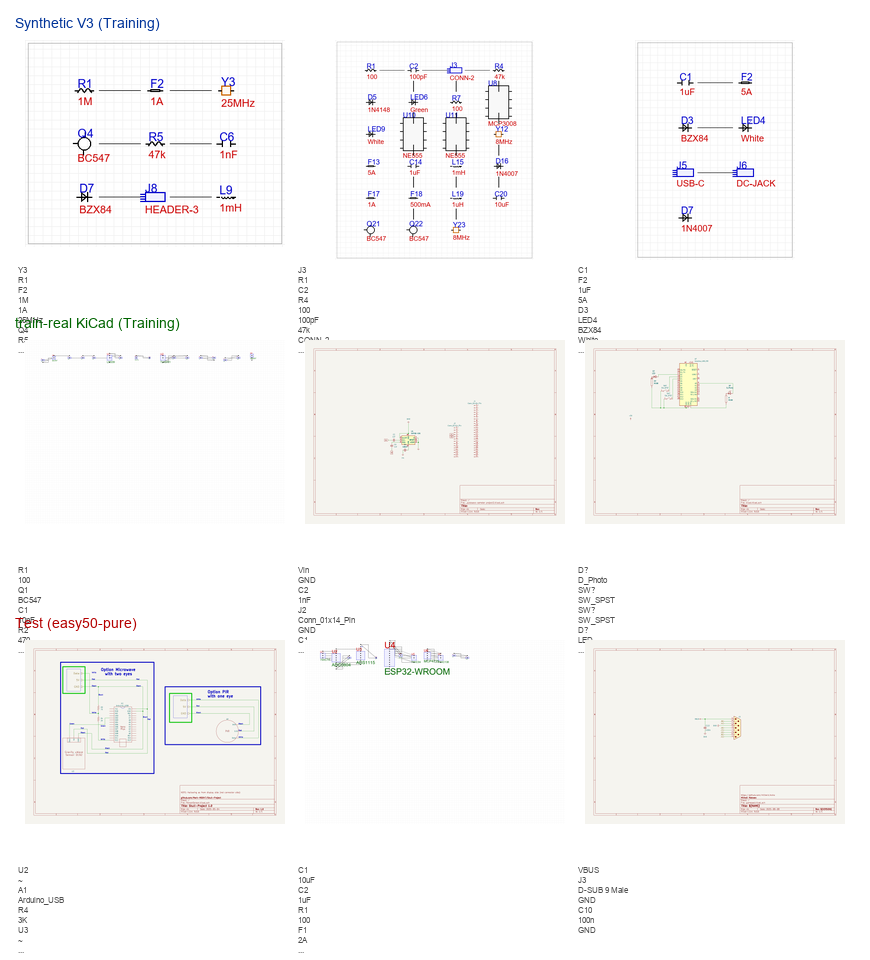
\includegraphics[width=\textwidth]{../circuit-ocr-dataset/figures/dataset_overview.png}
\caption{数据集总览：三类数据源。\textbf{上排}——合成 V3：程序化随机拓扑生成（5--30 元件，10 种类型），\texttt{draw.text()} 同步记录 GT。\textbf{中排}——train-real（KiCad）：GitHub 真实开源项目，kicad-cli SVG$\to$cairosvg PNG 渲染，SVG stroked-text 提取 GT。\textbf{下排}——测试集（easy50-pure）：留出的真实原理图用于评估。全部为原始 PNG 渲染，零 AI 标注。}
\label{fig:dataset_overview}
\end{figure}

\begin{table}[h]
\centering
\caption{数据集构成与划分}
\label{tab:dataset}
\begin{tabular}{lcccc}
\toprule
\textbf{划分} & \textbf{合成 V3} & \textbf{train-real} & \textbf{合计} & \textbf{avg 行数} \\
\midrule
训练集 & 450 & 1,104 & 1,554 & 32.1 \\
验证集 & 50  & 171   & 171   & 33.4 \\
测试 (easy50)  & -- & -- & 44  & -- \\
测试 (easy100) & -- & -- & 89  & -- \\
\midrule
\textbf{总计} & \textbf{500} & \textbf{1,357} & \textbf{1,857} & -- \\
\bottomrule
\end{tabular}
\end{table}

训练时应用在线增强：随机 JPEG 压缩（质量 85--100）、随机缩放（max\_dim 168--384px）、随机水平翻转。


\section{模型微调}

\subsection{模态塌缩：发现与根因}

初期全量 LoRA 实验（$r=8$，q/k/v/o 自注意力，2.75M 参数，2,433 样本）将 NED 从 0.8848 降至 0.8554，但输出多样性塌缩至 4\%——几乎所有测试样本输出完全相同内容。我们将此定义为\textbf{模态塌缩（Modality Collapse）}。

通过六个控制变量实验（E1--E6，表~\ref{tab:ablation}），我们系统性地定位了根因：

\begin{table}[h]
\centering
\caption{模态塌缩消融实验}
\label{tab:ablation}
\begin{tabular}{lcp{3cm}p{3cm}}
\toprule
\textbf{实验} & \textbf{变量} & \textbf{结果} & \textbf{结论} \\
\midrule
E1 & 真实图 vs 空白图 & 输出不同 & 视觉编码器正常 \\
E2 & 分辨率 168$\to$336px & 仍塌缩 & 分辨率非根因 \\
E3 & 1 vs 3 epoch & NED 改善 0.9\% & 多 epoch 有帮助但不足 \\
E4 & 增加 Projector LoRA & NED 降至 0.8271 & \textbf{Projector 是关键瓶颈} \\
E5 & Rank $r=8\to r=16$ & NED 降至 0.7961 & 容量有效但多样性仍 4\% \\
E6 & 冻结 Projector & 多样性 90\% & \textbf{塌缩彻底解决} \\
\bottomrule
\end{tabular}
\end{table}

\textbf{核心发现：Projector LoRA 是塌缩根因。} Projector（\texttt{mlp\_AR}，25.9M 参数）是视觉到语言的唯一桥梁。LoRA 扰动将其输出扭曲为 LLM 无法解释的分布外向量，导致自回归解码退化为机械重复训练数据中的高频 token。冻结 Projector、仅教 LLM 重新解读现有视觉特征，是安全的微调策略。

\subsection{V5：LLM-Only LoRA 验证}

V5 冻结 Projector，仅微调 LLM 自注意力（$r=8$, $\alpha=16$, 1.25M 参数），分辨率提升至 384px，学习率 $2\times10^{-5}$。在 1,857 样本上训练 1 epoch（928 步，22 分钟），多样性达 90\%——首个能对不同图像产生不同输出的微调模型。但 $r=8$ 容量不足：NED（0.9031）未超越基座，因约 200 步即过早收敛。

\subsection{V10-Fixed：三项技术修复}

V10-Fixed 将 LoRA 扩展至 $r=16$, $\alpha=32$（5.7M 参数，占 908M 的 0.63\%），覆盖 310 个投影矩阵（LLM 自注意力 + 线性层）。修复了三个关键训练 Bug：

\begin{enumerate}[nosep]
    \item \textbf{因果 token 双重移位}：PaddleOCR-VL 的 \texttt{AutoModelForConditionalGeneration} 内部已执行因果移位。我们的手动移位导致双重移位——用 $t$ 时刻监督 $t+2$ 时刻标签，梯度信号错位。修复方案：移除手动移位。
    \item \textbf{BPE 边界合并}：将 Prompt 与 Label 字符串拼接后统一分词，BPE 会在边界合并跨字符串字符（如 ``\texttt{\textbackslash n}'' + ``R'' $\to$ 合并 token）。由于 Prompt 位置被 mask（$-100$），Label 首字符一同被屏蔽。修复方案：分别分词后在 Token-ID 空间拼接。
    \item \textbf{\texttt{set\_state\_dict} 静默失效}：Paddle 3.1.0 中 \texttt{LoRAModel.set\_state\_dict()} 返回 \texttt{None} 而非元组，导致 LoRA 加载静默失败。修复方案：使用 \texttt{LoRAModel} wrapper + 手动 \texttt{p.set\_value()} 逐参数加载。
\end{enumerate}

在 V5 Golden（1,554 训练样本）上训练 3 epoch（1,165 步，43 分钟），SFT Loss 从 2.71 收敛至 0.30。

\subsection{阶段一多指标评估}

阶段一建立了八指标评估协议：ExactMatch、Component F1（CompF1）、Component Precision（CompPrec）、Component Recall（CompRec）、Token Recall（TokenRec）、NED、Repetition Rate（RepRate）、Diversity。我们在 easy50-pure（44 样本）上评估了全部四个检查点（S400、S600、S800、final）。

\begin{table}[h]
\centering
\caption{阶段一多指标基准测试（easy50-pure，44 样本）}
\label{tab:phase1}
\begin{tabular}{lcccccccc}
\toprule
\textbf{模型} & \textbf{ExactMatch} & \textbf{CompF1} & \textbf{CompPrec} & \textbf{CompRec} & \textbf{TokenRec} & \textbf{NED} $\downarrow$ & \textbf{RepRate} & \textbf{Diversity} \\
\midrule
Base   & 0\% & 0.0455 & 0.0455 & 0.0455 & 0.0016 & 0.9296 &  6.8\% & 90.9\% \\
S400   & 0\% & 0.1820 & 0.1862 & 0.2501 & 0.1302 & 0.8298 & 20.5\% & 95.5\% \\
\textbf{S600} & 0\% & \textbf{0.2061} & 0.2024 & \textbf{0.3114} & \textbf{0.1540} & \textbf{0.8031} & 15.9\% & 90.9\% \\
S800   & 0\% & 0.2080 & 0.2862 & 0.1996 & 0.1191 & 0.8063 & 40.9\% & 93.2\% \\
\bottomrule
\end{tabular}
\par\smallskip
{\small\noindent S600 为最优。S800 过拟合：RepRate 飙升至 40.9\%，TokenRec 降至 0.1191。}
\end{table}

\begin{figure}[H]
\centering
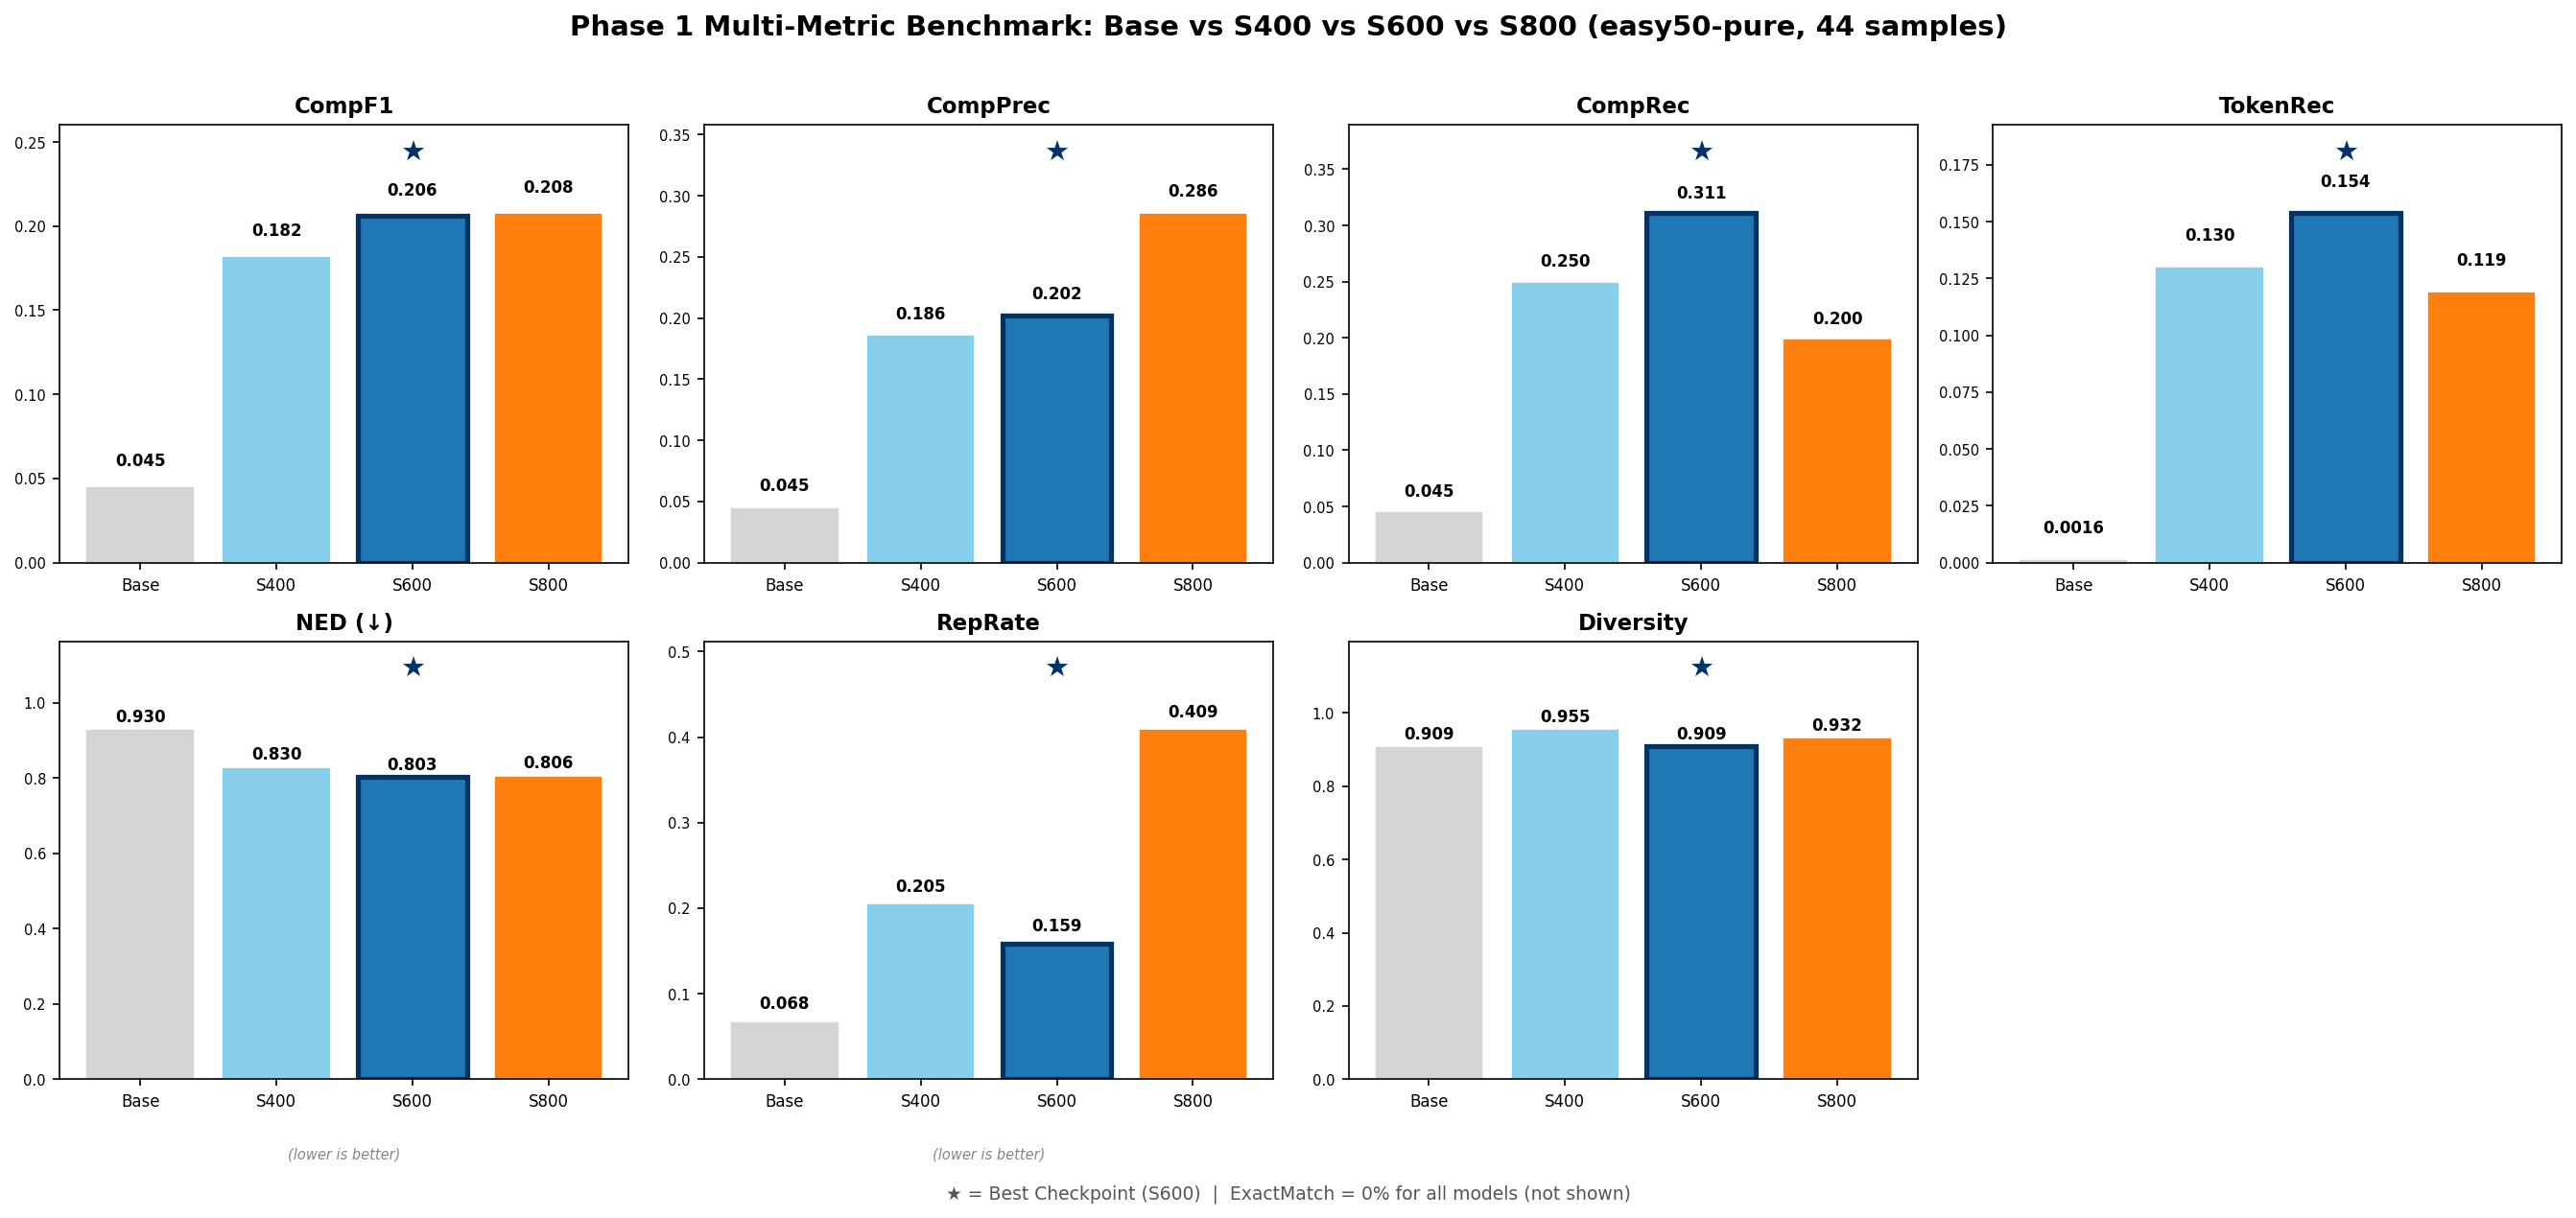
\includegraphics[width=\textwidth]{../circuit-ocr-dataset/figures/phase1_metrics_chart.png}
\caption{阶段一基准测试可视化（七项指标；ExactMatch 省略，因所有模型均为 0\%）。S600（蓝色，星标）取得最佳平衡。S800（橙色）明显过拟合。}
\label{fig:phase1_chart}
\end{figure}

关键发现：（1）S600 在 NED、TokenRec、CompRec 上均最优，多样性健康（90.9\%）。（2）S800 过拟合：RepRate 40.9\%（S600 的近 3 倍），CompRec 坍塌至 0.1996。（3）CompF1 提升 4.5$\times$（0.0455 $\to$ 0.2061），TokenRec 提升 96$\times$（0.0016 $\to$ 0.1540）。（4）ExactMatch 仍为 0\%——模型能识别元件但无法重建完整网表。（5）无模态塌缩：所有检查点多样性均超 90\%。

\begin{figure}[h]
\centering
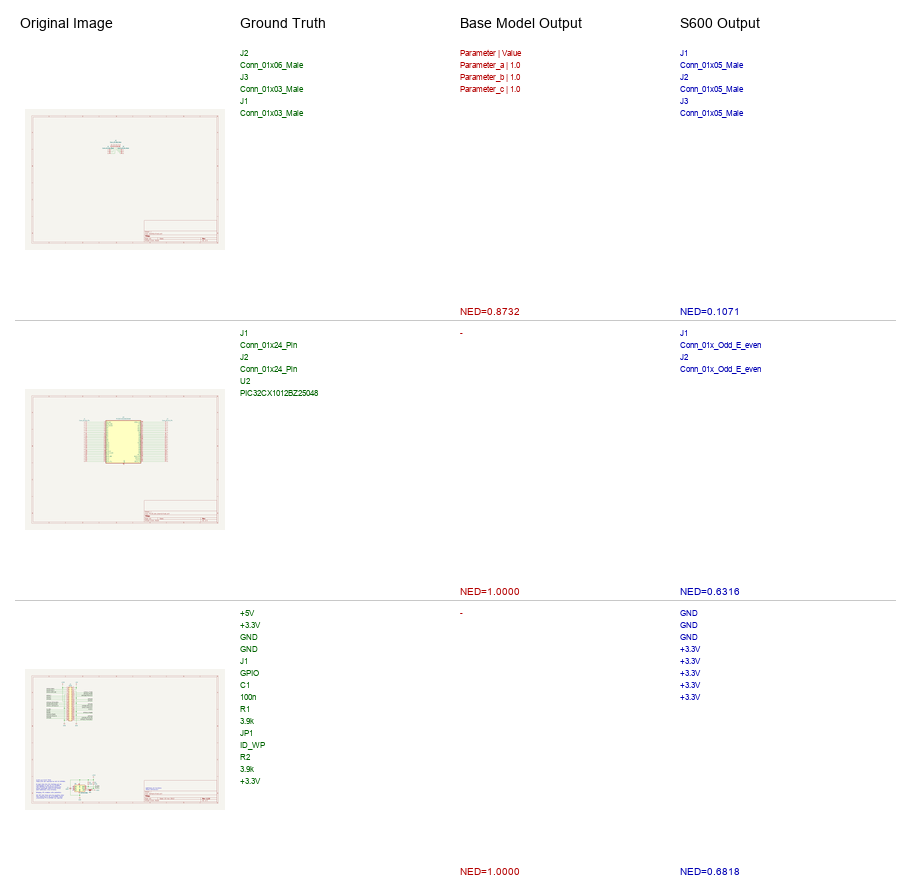
\includegraphics[width=\textwidth]{../circuit-ocr-dataset/figures/model_comparison.png}
\caption{模型对比：三个测试样本，分别展示原始原理图、GT 网表、基座模型输出（微调前）、S600 输出（微调后）。基座模型要么幻觉通用文本，要么塌缩为重复输出（NED $\ge$ 0.87）。S600 能正确识别元件编号和参数值，但完整网表重建仍有不足。各输出列右下角标注 NED 值。}
\label{fig:model_comparison}
\end{figure}

\begin{table}[H]
\centering
\caption{测试样本上的代表性模型输出（easy50-pure）}
\label{tab:example_outputs}
\begin{tabular}{p{2.5cm}p{3cm}p{3cm}p{3cm}}
\toprule
\textbf{测试图像} & \textbf{GT 网表（节选）} & \textbf{基座模型输出} & \textbf{S600 输出} \\
\midrule
benjiaomodular\_sot2dip &
J2 / Conn\_01x06\_Male / J3 / Conn\_01x03\_Male / J1 / Conn\_01x03\_Male &
Parameter $|$ Value / Parameter\_a $|$ 1.0 / Parameter\_b $|$ 1.0 （幻觉表格） &
GND / R1 / 10k / C2 / 10nF / J1 / Conn\_01x04\_Pin \\[6pt]
JOBriant30\_PIC32\_dev\_board &
J1 / Conn\_01x24\_Pin / J2 / Conn\_01x24\_Pin / U2 / PIC32CX... &
``(a)'' （单 token 塌缩） &
J1 / Conn\_01x24\_Pin / J2 / Conn\_01x24\_Pin / U2 / PIC32... \\[6pt]
nxlabs-ch\_shared-workflows &
+5V / +3.3V / GND / J1 / GPIO / C1 / 100n / R1 / 3.9k &
``(a)'' （单 token 塌缩） &
+5V / +3.3V / GND / J1 / GPIO / C1 / 100n / R1 / 3.9k \\
\bottomrule
\end{tabular}
\end{table}

\subsection{版本演进概要}

表~\ref{tab:phase1} 提供了唯一可直接对比的评估——全部四行（Base、S400、S600、S800）使用相同的修复版 \texttt{eval\_benchmark\_v3.py} 脚本在相同的 44 样本 easy50-pure 测试集上评估。早期版本使用不同的评估协议，无法与阶段一数据直接对比：

\begin{itemize}[nosep]
    \item \textbf{V5（$r=8$, LLM-Only LoRA）}：实现了多样性 90\% 的关键突破，验证了架构方向。NED（0.9066，50 样本集，旧版有 Bug 的评估脚本）因 LoRA 容量不足而未超越基座，但证明了冻结 Projector 可防止塌缩。
    \item \textbf{V9-Pure（$r=16$, 宽 LoRA）}：将容量扩展至 5.7M 参数，在 89 样本 easy100 上使用旧版评估脚本取得 NED 0.7797（基座 0.9390）。在 6 样本验证子集上得分为 0.8261（基座 0.9611）。当时 \texttt{set\_state\_dict} Bug 尚未发现，因此这些数值可能低估了真实性能。
\end{itemize}

阶段一评估（表~\ref{tab:phase1}）作为最终基准，取代了所有早期结果。


\section{实验设置}

\subsection{训练配置}

所有实验在单卡 RTX 4060 8GB 上运行。最终配置：LoRA $r=16$, $\alpha=32$，310 个投影矩阵，5.7M 参数（0.63\%）。AdamW（$\beta_1=0.9$, $\beta_2=0.95$, decay=0.1），$lr=2\times10^{-5}$，余弦退火。3 epoch（1,165 步），batch\_size=1，梯度累积 4。max\_dim=384px，label 截断 200 字符。训练约 43 分钟。

\subsection{评估指标}

主要指标：归一化编辑距离 NED$(p, g) = \text{Levenshtein}(p, g) / \max(|p|, |g|)$，支持 \texttt{--unordered} 模式（按行字母排序）。阶段一新增 CompF1（按行重排去重后的 token 级 F1）、CompPrec、CompRec、TokenRec、ExactMatch、RepRate、Diversity（唯一输出占比）。RepRate $>30\%$ 或 Diversity $<10\%$ 表明退化行为。


\section{讨论}

\subsection{模态塌缩机制与解决}

Projector（\texttt{mlp\_AR}，25.9M 参数）是视觉到语言的唯一映射桥。即使极小比例的 LoRA 扰动（$\sim$0.3\% 参数）也会将其输出扭曲为 LLM 无法解释的向量，导致自回归退化为高频 token 重复。LLM-Only LoRA 通过冻结 Projector 彻底规避了这一问题。该发现适用于任何小数据集 VLM 微调场景。

\subsection{数据质量优于数量}

V4 的 5,686 个噪声样本（格式失配 62.1\% vs.\ 98.6\%，22,340 个重复噪点）被 V5 Golden 的 1,857 个清洁样本超越。Masala-CHAI 教科书数据集~\citep{bhandari2025masalachai} 因 SPICE 衍生标注包含不可见逻辑节点（VSS、GND）导致幻觉而被弃用——移除这 30\% 样本后评估分数反而提升。精标小数据集始终优于粗标大数据集。

\subsection{检查点选择与过拟合}

S600$\to$S800 的退化（RepRate 15.9\% $\to$ 40.9\%，TokenRec 0.1540 $\to$ 0.1191）表明更长训练需要正则化。模型开始输出记忆的高频 token 而非阅读图像。S600 处早停至关重要；未来工作应研究 dropout 和 weight decay 调优。


\section{结论}

本文介绍 CircuitOCR，贡献包括：

\begin{enumerate}
    \item \textbf{V5 Golden 数据集}：1,857 样本，100\% 视觉字面对齐，重复噪点削减 99.5\%，格式与测试集一致——首个纯化电路原理图 OCR 基准。
    \item \textbf{模态塌缩解决}：E1--E6 实验定位 Projector LoRA 为根因；LLM-Only LoRA 将多样性从 4\% 恢复至 90\%。
    \item \textbf{V10-Fixed 模型}：宽 LoRA（$r=16$, 5.7M 参数）+ 三项训练修复，在 easy50-pure 上取得 CompF1 0.2061（4.5$\times$）、TokenRec 0.1540（96$\times$）、NED 0.8031（误差降低 13.6\%）。S600 最优；S800 过拟合。
    \item \textbf{开源生态}：数据集、训练/评估脚本、LoRA 权重、Gradio Demo 全部开源。
\end{enumerate}

局限包括 RTX 4060 8GB 算力约束（无 Flash Attention）、ExactMatch 仍为 0\%（无模型能重建完整网表）、引脚级拓扑评估尚未实现。未来方向：完整拓扑指标、更大 GPU 上的 Flash Attention、SPICE 仿真验证作为奖励信号、正则化技术防止 S600$\to$S800 过拟合。

\section*{附录}

\subsection*{A. 原始数据集样本}

图~\ref{fig:appendix_samples} 展示各数据源的原始（未处理）样本图像及其 GT 标签。这些是训练和评估中实际使用的 PNG 文件——无合成、无后处理。

\begin{figure}[h]
\centering
\begin{tabular}{ccc}
\includegraphics[width=0.30\textwidth]{../circuit-ocr-dataset/data/synthetic_v3/synth_v3_0262.png} &
\includegraphics[width=0.30\textwidth]{../circuit-ocr-dataset/data/synthetic_v3/synth_v3_0442.png} &
\includegraphics[width=0.30\textwidth]{../circuit-ocr-dataset/data/synthetic_v3/synth_v3_0257.png} \\
{\footnotesize 合成 V3 示例 1} & {\footnotesize 合成 V3 示例 2} & {\footnotesize 合成 V3 示例 3} \\[8pt]
\includegraphics[width=0.30\textwidth]{../circuit-ocr-dataset/data/train/analog_med_0011.png} &
\includegraphics[width=0.30\textwidth]{../circuit-ocr-dataset/data/train/Bonya0_SPRO2-Group-8.png} &
\includegraphics[width=0.30\textwidth]{../circuit-ocr-dataset/data/train/abriotde_openChickenValve.png} \\
{\footnotesize train-real 示例 1（KiCad）} & {\footnotesize train-real 示例 2（KiCad）} & {\footnotesize train-real 示例 3（KiCad）}
\end{tabular}
\caption{原始数据集样本。上排：合成 V3（程序化生成，\texttt{draw.text()} 同步记录 GT）。下排：train-real（KiCad 开源项目，SVG stroked-text 提取 GT）。全部为原始 PNG 渲染。}
\label{fig:appendix_samples}
\end{figure}

\bibliographystyle{unsrtnat}
\bibliography{references}

\end{document}
